\subsection{Inductive limits of sequences of locally convex spaces}

In this No.~we shall consider an increasing sequence \((\mathrm{E}_{n})\) of vector subspaces of a vector space E, such that E is the union of the \(E_{n}\) ; we suppose that each \(E_{n}\) carries a locally convex topology \(\mathcal{T}_n\) , such that, for every \(n\) , the topology induced on \(\mathrm{E}_n\) by \(\mathcal{T}_{n+1}\) is coarser than \(\mathcal{T}_n\) , and we give to E the locally convex topology \(\mathcal{T}\) that is the inductive limit of the sequence \((\mathcal{T}_n)\) (II, p.~29, Example II); these hypotheses and notations will be used throughout the rest of this No.~without restatement.

It may happen that each \(T_{n}\) is Hausdorff but that T is not; it may also happen that for each pair of integers n, m such that \(n \leqslant m\) , the subspace \(E_{n}\) is closed in \(E_{m}\) (using topology \(T_{m}\) ) but that \(E_{n}\) is not closed in E using T (II, p.~80, exerc. 26).

Lemma 1. --- Let F be a Cauchy filter on E (for T); then there exists an integer k, such that for all \(N \in F\) and every neighbourhood V of 0 in E, the subspace \(E_{k}\) meets \(N + V\) .

We assume the contrary and obtain a contradiction. Suppose that for every \(k\) there exists a convex neighbourhood \(\mathbf{V}_k\) of 0 and a set \(\mathbf{M}_k \in \mathfrak{F}\) such that

\[
\left(\mathrm{E} _ {k} + \mathrm{V} _ {k}\right) \cap \mathrm{M} _ {k} = \varnothing .
\]

Clearly we can suppose that \(\mathrm{V}_{k + 1} \subset \mathrm{V}_k\) for all \(k\) . Let \(\mathbf{V}\) be the convex envelope of \(\bigcup_{k} (\mathrm{E}_k \cap \mathrm{V}_k)\) , this is clearly a neighbourhood of 0 for \(\mathcal{T}\) . For all \(n\) we have \(\mathbf{V} \subset \mathbf{V}_n + \mathbf{E}_n\) ; in fact, every \(x \in \mathbf{V}\) can be written \(\sum_{i} \lambda_i x_i\) where \(\lambda_i \geqslant 0\) , \(\sum_{i} \lambda_i = 1\) and \(x_i \in \mathrm{V}_i \cap \mathrm{E}_i\) for all \(i\) ; now for \(i < n\) we have \(x_i \in \mathrm{E}_n\) , therefore \(\sum_{i < n} \lambda_i x_i \in \mathrm{E}_n\) ; and for \(i \geqslant n\) we have \(x_i \in \mathrm{V}_n\) , therefore \(\sum_{i \geqslant n} \lambda_i x_i \in \mathrm{V}_n\) since \(\mathrm{V}_n\) is convex, contains 0 and \(\sum_{i \geqslant n} \lambda_i \leqslant 1\) . Hence \(\mathrm{V} + \mathrm{E}_n \subset \mathrm{V}_n + \mathrm{E}_n\) for all \(n\) . This being so, let \(\mathbf{M} \in \mathfrak{F}\) be a set that is V-small. For some integer \(m\) , \(\mathrm{E}_m \cap \mathbf{M}\) is not empty; and we conclude that

\[
\mathbf {M} \subset \mathrm{E} _ {m} + \mathrm{V} \subset \mathrm{E} _ {m} + \mathrm{V} _ {m};
\]

as \(\mathfrak{F}\) is a filter, the set \(\mathbf{M}_m\) meets \(\mathbf{M}\) and therefore \(\mathrm{E}_m + \mathrm{V}_m\) ; we have a contradiction which establishes the lemma.

PROPOSITION 9. --- Suppose that the topology induced on \(\mathbf{E}_n\) by \(\mathcal{T}_{n+1}\) is identical with \(\mathcal{T}_n\) for every integer \(n\) . Then

\begin{enumerate}
\def\labelenumi{(\roman{enumi})}
\item
  The topology induced by \(\mathcal{T}\) on \(\mathbf{E}_n\) is identical with \(\mathcal{T}_n\) for each \(n\) ; if the \(\mathcal{T}_n\) are Hausdorff then \(\mathcal{T}\) is Hausdorff.
\item
  If, for every \(n\) , \(\mathbf{E}_n\) is closed in \(\mathbf{E}_{n+1}\) (for \(\mathcal{T}_{n+1}\) ), then \(\mathbf{E}_n\) is closed in \(\mathbf{E}\) (using \(\mathcal{T}\) ) for every \(n\) .
\item
  If each \(\mathrm{E}_n\) is complete (using \(\mathcal{T}_n\) ) then \(\mathrm{E}\) is complete using \(\mathcal{T}\) .
\item
  To prove the first assertion, it is sufficient to prove that the topology \(\mathcal{T}_n'\) induced by \(\mathcal{T}\) on \(\mathrm{E}_n\) is finer than \(\mathcal{T}_n\) . For this, let \(\mathrm{V}_n\) be a convex neighbourhood of 0 in \(\mathrm{E}_n\) for the topology \(\mathcal{T}_n\) ; we are going to construct an increasing sequence of convex neighbourhoods of 0 in \(\mathrm{E}_{n+p}\) for \(\mathcal{T}_{n+p}\) , say \((\mathrm{V}_{n+p})_{p\geqslant 1}\) , such that \(\mathrm{V}_{n+p} \cap \mathrm{E}_n = \mathrm{V}_n\) for every index \(p \geqslant 1\) . Then the union V of the increasing sequence \((\mathrm{V}_{n+p})\) will be a convex set such that \(\mathrm{V} \cap \mathrm{E}_k\) is a neighbourhood of 0 in \(\mathrm{E}_k\) (using \(\mathcal{T}_k\) ), for every index \(k\) ; therefore V will be a neighbourhood of 0 in E for \(\mathcal{T}\) and as \(\mathrm{V} \cap \mathrm{E}_n = \mathrm{V}_n\) , we have proved that \(\mathcal{T}_n'\) is finer than \(\mathcal{T}_n\) .
\end{enumerate}

To define the \(\mathrm{V}_{n + p}\) we proceed by induction on \(p\) using the following lemma:

Lemma 2. --- Let V be a convex neighbourhood of 0 in M, a vector subspace of a locally convex space F. Then there exists a convex neighbourhood W of 0 in F such that \(W \cap M = V\) . Further, if M is closed in F, then, for every point \(x_{0} \in C M\) , there exists a convex neighbourhood \(W_{0}\) of 0 in F such that \(W_{0} \cap M = V\) and \(x_{0} \notin W_{0}\) .

In fact, by hypothesis there exists a convex neighbourhood U of 0 in F such that \(U \cap M \subset V\) . Clearly, the convex envelope W of \(U \cup V\) in F is a neighbourhood of 0 in F; we show that \(W \cap M = V\) . For, every point \(z \in W\) is of the form \(\lambda x + (1 - \lambda)y\) with \(x \in V\) , \(y \in U\) , and \(0 \leqslant \lambda \leqslant 1\) (II, p.~9, prop. 8); if \(z \in M\) , and \(\lambda \neq 1\) then necessarily \(y \in M\) , therefore \(y \in U \cap M \subset V\) and hence \(z \in V\) ; the result is obviously true if \(\lambda = 1\) . If M is closed in F, the space F/M is Hausdorff, thus there exists a convex neighbourhood \(U_0 \subset U\) of 0 in F such that \(U_0\) does not meet \(x_0 + M\) ; then the convex envelope \(W_0\) of \(U_0 \cup V\) fulfils the required conditions.

Returning to the theorem, to prove the second part of (i) note that if \(x \in E\) then \(x \in E_n\) for some \(n\) ; if \(x \neq 0\) and \(\mathcal{T}_n\) is Hausdorff then there is a neighbourhood \(V_n\) of 0 for \(\mathcal{T}_n\) , which does not contain \(x\) . We see that there is a neighbourhood \(V\) of 0 for \(\mathcal{T}\) such that \(V \cap E_n = V_n\) , hence \(x \notin V\) , and it follows that \(\mathcal{T}\) is Hausdorff.

\begin{enumerate}
\def\labelenumi{(\roman{enumi})}
\setcounter{enumi}{1}
\item
  Let \(x \in \mathrm{E} - \mathrm{E}_n\) ; there exists \(m > n\) such that \(x \in \mathrm{E}_m\) , thus, as \(\mathrm{E}_n\) is closed in \(\mathrm{E}_m\) for \(\mathcal{T}_m\) (because of the hypothesis that \(\mathcal{T}_{n+1}\) induces \(\mathcal{T}_n\) on \(\mathrm{E}_n\) for every \(n\) ) there exists in the topology \(\mathcal{T}_m\) a convex neighbourhood \(\mathrm{V}_m\) of 0 in \(\mathrm{E}_m\) such that \((x + \mathrm{V}_m) \cap \mathrm{E}_n\) is empty. Now we saw in (i) that there exists a convex neighbourhood \(\mathrm{V}\) of 0 for \(\mathcal{T}\) such that \(\mathrm{V} \cap \mathrm{E}_m = \mathrm{V}_m\) ; and thus \((x + \mathrm{V}) \cap \mathrm{E}_m = x + \mathrm{V}_m\) , therefore \((x + \mathrm{V}) \cap \mathrm{E}_n = \emptyset\) , which proves (ii).
\item
  From lemma 1, if \(\mathfrak{F}\) is a minimal Cauchy filter for \(\mathcal{T}\) (GT, II, §3.2) then there exists a \(k\) such that the trace of \(\mathfrak{F}\) on \(\mathrm{E}_k\) is a filter \(\mathfrak{F}_k\) ; from (i) this last is a Cauchy filter for \(\mathcal{T}_k\) and thus \(\mathfrak{F}_k\) converges in \(\mathrm{E}_k\) by hypothesis; but as the filter on E generated by \(\mathfrak{F}_k\) is finer than \(\mathfrak{F}\) , we see that \(\mathfrak{F}\) has a cluster point for \(\mathcal{T}\) and thus converges for \(\mathcal{T}\) .
\end{enumerate}

When for all \(n\) the topology induced on \(\mathbf{E}_n\) by \(\mathcal{T}_{n+1}\) is just \(\mathcal{T}_n\) we say that \(\mathcal{T}\) is the strict inductive limit of the sequence \((\mathcal{T}_n)\) and that the space \(\mathbf{E}\) with the topology \(\mathcal{T}\) is the strict inductive limit of the sequence of locally convex spaces \(\mathbf{E}_n\) .

Remarks. --- 1) Suppose that E is the union of an increasing directed, non-enumerable family of subspaces \((\mathrm{E}_{\alpha})_{\alpha \in I}\) , each \(\mathrm{E}_{\alpha}\) having a locally convex topology \(\mathcal{T}_{\alpha}\) , such that, for \(\mathrm{E}_{\alpha} \subset \mathrm{E}_{\beta}\) , the topology induced on \(\mathrm{E}_{\alpha}\) by \(\mathcal{T}_{\beta}\) is identical with \(\mathcal{T}_{\alpha}\) . It may be the case that the topology induced on each \(\mathrm{E}_{\alpha}\) by the topology \(\mathcal{T}\) is equal to \(\mathcal{T}_{\alpha}\) and that the \(\mathrm{E}_{\alpha}\) are Hausdorff and complete, but that E is not complete for \(\mathcal{T}\) (INT, III, 2nd ed., § 1, exerc. 2).

\pandocbounded{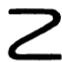
\includegraphics[keepaspectratio]{images/part001_ec6127c7.jpg}}

\begin{enumerate}
\def\labelenumi{\arabic{enumi})}
\setcounter{enumi}{1}
\item
  Let \(\mathbf{F}\) be a locally convex space, which is the union of an increasing sequence of vector subspaces \((\mathbf{F}_n)\) , and for each index \(n\) , let \(\mathcal{T}_n\) be the topology induced on \(\mathbf{F}_n\) by the topology \(\mathcal{T}\) of \(\mathbf{F}\) . One should beware that in general \(\mathcal{T}\) is not the inductive limit of the \(\mathcal{T}_n\) .
\item
  Suppose that \(\mathbf{E}\) is the strict inductive limit of the sequence \((\mathbf{E}_n)\) ; if \(\mathbf{F}\) is a closed (in \(\mathcal{T}\) ) vector subspace of \(\mathbf{E}\) , it may be the case that the strict inductive limit of the topologies induced by the \(\mathcal{T}_n\) on \(\mathrm{F} \cap \mathrm{E}_n\) is strictly finer than the topology induced by \(\mathcal{T}\) (IV, p.~63, exerc. 10).
\end{enumerate}

PROPOSITION 10. --- Let E, F be two locally convex spaces. Suppose that :

\begin{enumerate}
\def\labelenumi{\arabic{enumi})}
\item
  There exists a family of Fréchet spaces \((\mathbf{E}_{\alpha})\) , and for each \(\alpha\) a linear mapping \(g_{\alpha}: \mathbf{E}_{\alpha} \to \mathbf{E}\) , such that the topology of \(\mathbf{E}\) is the final locally convex topology for the family \((g_{\alpha})\) .
\item
  There exists a sequence of Fréchet spaces \((\mathbf{F}_n)\) and for each \(n\) a continuous linear injection \(j_n: \mathbf{F}_n \to \mathbf{F}\) such that \(\mathbf{F} = \bigcup j_n(\mathbf{F}_n)\) .
\end{enumerate}

Then every linear mapping \(u\) of \(\mathbf{E}\) in \(\mathbf{F}\) , whose graph is closed in \(\mathbf{E} \times \mathbf{F}\) , is necessarily continuous.

To prove that u is continuous, it is sufficient to show that for every \(\alpha\) , the mapping \(u \circ g_{\alpha}: E_{\alpha} \to F\) is continuous (II, p.~27, prop. 5). Now the graph of \(u \circ g_{\alpha}\) is the inverse image of the graph of u under the continuous mapping \(g_{\alpha} \times 1_{F}: E_{\alpha} \times F \to E \times F\) , and therefore is, by hypothesis, closed in \(E_{\alpha} \times F\) . We can, therefore, restrict ourselves to the case when E itself is a Fréchet space. But then the proposition is a particular case of I, p.~20, prop. 1.

COROLLARY. --- With the same hypotheses on E and F as in prop. 10 and assuming that E is Hausdorff, then every continuous surjective mapping v of F in E is a strict morphism.

Let N be the kernel of v and write \(\mathrm{N}_{n}=j_{n}^{-1}(\mathrm{N})\) ; then the mapping \(j_{n}^{\prime}:F_{n}/N_{n}\to F/N\) , deduced from \(j_{n}\) by taking quotients, is injective and continuous, also \(F_{n}/N_{n}\) is a Fréchet space (since \(N_{n}\) is closed) and F/N is the union of the images under \(j_{n}^{\prime}\) . By hypothesis, in the canonical factorisation \(v:F\to F/N\stackrel{w}{\to}E\) , the linear mapping w is bijective and continuous and its graph in \((\mathrm{F/N})\times\mathrm{E}\) is therefore closed (GT, I, §8.1, cor. 2 of prop. 2). By the remarks at the beginning and by prop. 10, the inverse mapping u of w is therefore continuous and the corollary is proved.

* Prop. 10 and its corollary apply in particular when E is a complete bornological space (III, p.~12) and F is the inductive limit of a sequence of Fréchet spaces.*

